\chapter{The Large Hadron Collider}
The Large Hadron Collider (LHC) \cite{LHC_machine} is a 26.7km long circular superconducting high-energy particle accelerator, located approximately 100m underground near the city of Geneva, Switzerland. The LHC occupies the tunnel constructed between 1984 and 1989 for the Large Electron-Positron Collider. It also borrows some injection infrastructure from the LEP machine. The LHC is operated by the European Organization for Nuclear Research (CERN), the largest international scientific collaboration in the world.\\

The LHC accelerates protons and heavy ions and collides them at four interaction points around the ring, with a design center-of-mass energy per collision of $\sqrt{s}$ = 14 TeV. Each interaction point is home to one of four detector experiments, which study the products of the collisions. The largest of these experiments is the ATLAS detector \cite{ATLAS_at_LHC}, a general purpose detector for studying the Standard Model and searching for physics beyond it. The CMS detector \cite{CMS_at_LHC}is another general purpose detector, designed and operated independently of the ATLAS detector, but intended to probe the same range of physics. The ALICE \cite{ALICE_at_LHC} experiment is a dedicated heavy ion experiment, and the LHC-b \cite{LHCb_at_LHC} experiment is a dedicated $b$-physics experiment.\\

The first proton-proton collisions at the LHC were achieved in 2010 at a center-of-mass energy of $\sqrt{s}$ = 7 TeV. Run 1 of the LHC took place between 2010 and 2013. The data collected during this time led to the announcement of the discovery of the Higgs Boston in 2012 \cite{higgs_paper}. Between 2013 and 2015 the LHC underwent the first Long Shutdown (LS1) during which time key upgrades to the physics detectors and the accelerator chain were installed. Run 2 of the LHC was active from 2015 to 2018 and achieved a center-of-mass energy of $\sqrt{s}$ = 13 TeV. Between 2018 and 2022 the LHC underwent the second Long Shutdown (LS2). Run-3 of the LHC began in 2022 and achieved a a center-of-mass energy of $\sqrt{s}$ = 13.6 TeV.

 \section{Accelerator Physics}
 \subsection{The Journey of a Proton}
 Protons which feed the LHC start as hydrogen gas. The electrons are removed from the hydrogen atoms through the use of strong electric fields. The linear accelerator (LINAC) then accelerates the $H^-$ ions to an energy of 50 MeV. From here the $H^-$ ions enter the Proton Synchrotron booster, where they are accelerated up to 1.4 GeV of energy. Subsequently they are sorted into bunches separated in time by 25 ns,  where each bunch contains approximately $10^11$ protons. Next the bunches pass through the Proton Synchrotron (PS) and the Super Proton Synchrotron (SPS), where they reach energies of 25 GeV and 450 GeV respectively. Finally they are injected into the LHC as two beams traveling in opposite direction, and can be accelerated up to 7 TeV of energy. Due to limitations with the magnet training, the highest energy actually achieved by the LHC beams during Run 2 was 6.5 TeV each, giving a collision center-of-mass energy of $\sqrt{s}$ = 13 TeV. Figure \ref{fig:accelerator_complex} shows the full LHC accelerator complex.\\

\begin{figure}
	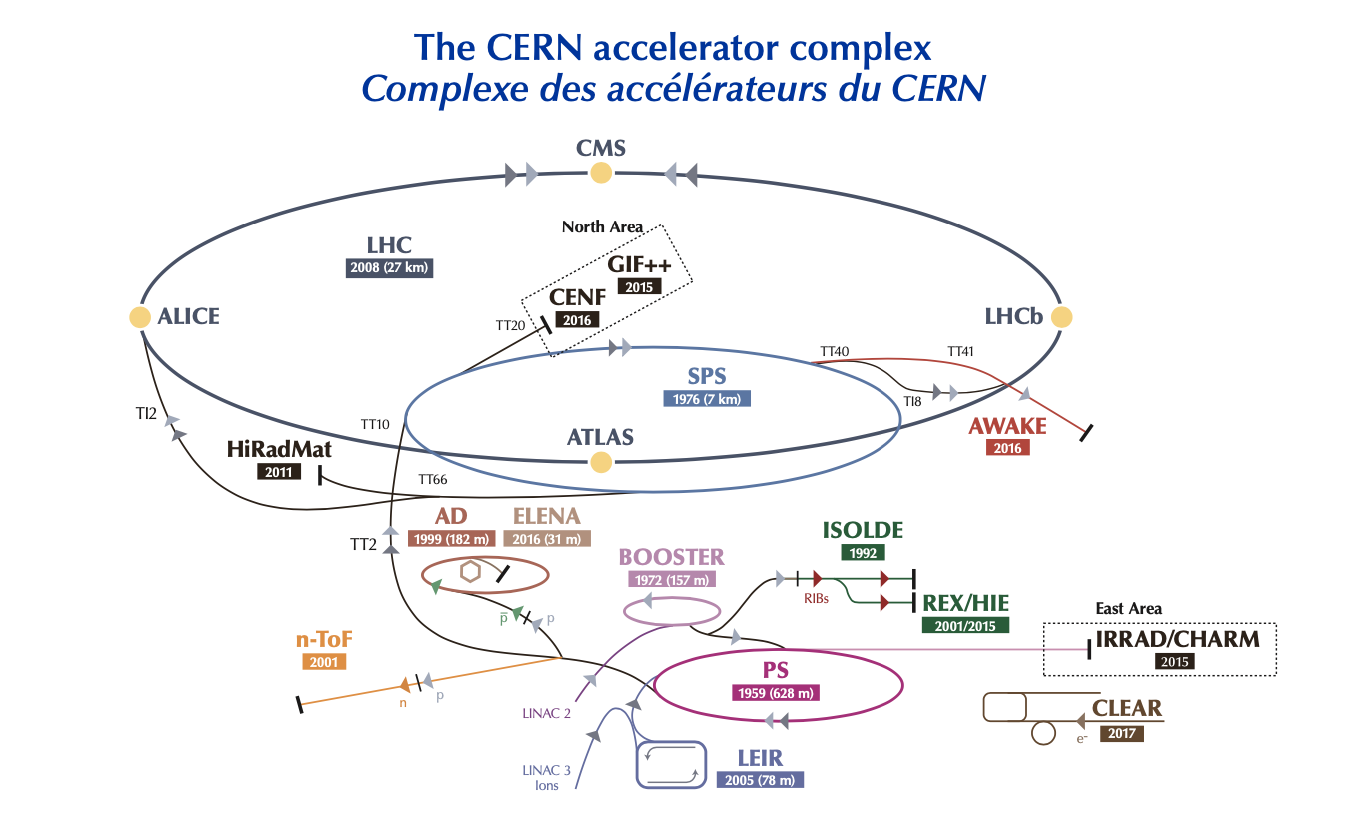
\includegraphics[width=\textwidth]{figures/accelerator_complex.png}
	\caption{The LHC accelerator complex at CERN \cite{cern_accelerator_complex}}
	\label{fig:accelerator_complex}
\end{figure}

 Acceleration in the LHC is performed by eight radio frequency (RF) cavities located around the ring. Each RF cavity produces a 2MV electric field oscillating at 40 MHz. This oscillation is synchronized with the occurrence of the proton bunches produced in the PS. The 40MHz oscillation produces points of stable equilibrium every 2.5ns -- a proton bunch occupies this point of stable equilibrium one out of every ten times, such that the bunches maintain their 25ns spacing. This is illustrated in figure \ref{fig:rf_buckets}. \\
 
 \begin{figure}
	\includegraphics[width=\textwidth]{figures/rf_buckets.png}
	\caption{The LHC accelerator complex at CERN}
	\label{fig:rf_buckets}
\end{figure}
 
In addition to the acceleration cavities, the LHC houses 9593 superconducting electromagnets which direct and focus the proton beam on it's 27km journey. The magnets are comprised of superconducting Niobium-Titanium coils cooled by superfluid helium at 1.4 K. As the beams approach one of the four collision points around the ring, additional multipole magnets focus and squeeze the beam for optimal collisions.\\
 
  \subsection{Luminosity}
 
Collisions at the LHC occur when the two beams of proton bunches cross at one of the four interaction points. The intensity of collisions is described by the instantaneous luminosity, the formula for which is given in equation \ref. The instantaneous luminosity gives the number of the collisions that could be produced at the interaction point per $cm^2$ of cross-sectional area per second. The integrated luminosity is obtained by integrating the instantaneous luminosity over time, and measures the total number of collisions which has occurred over the course of running. This is directly correlated with the size of the datasets collected by the LHC experiments. 
 
 \begin{equation}
	\L = \frac{N_1 N_2}{4 \pi \sigma_x \sigma_y}
	\label{eq:lumi}
\end{equation}
 
 The design peak luminosity of the LHC is $1.0 \times 10^34 cm^-2 s^-1$. During Run 1 of the LHC the peak instantaneous luminosity achieved was $0.8 \times 10^34 cm^-2 s^-1$. Over the course of Run 1 the LHC collected a total integrated luminosity of  $5.46 fb^-1$ at $\sqrt{s} = 7 TeV$, and $22.8 fb^-1$ at $\sqrt{s} = 8 TeV$. Following the first long shutdown and upgrade phase of operations, the LHC achieved a center of mass energy $\sqrt{s} = 13 TeV$ at the beginning of Run 2 in 2015. The LHC was also able to deliver $2.0 x 10^34 cm^-2 s^-1$ peak instantaneous luminosity, double the design value. During LHC Run 2, from 2015-2018, the LHC delivered $\L = 156 fb^-1$
 of integrated luminosity for proton-proton collisions. Run 3 of the LHC began in 2022, and is expected to deliver $250 fb^-1$ of integrated luminosity to the ATLAS and CMS experiments by 2026.\\
 
